\documentclass{article}
\usepackage[pdftex,
        colorlinks=true,
        urlcolor=rltblue,       % \href{...}{...} external (URL)
        filecolor=rltgreen,     % \href{...} local file
        linkcolor=rltred,       % \ref{...} and \pageref{...}
        pdftitle={Phys 20 Lab 4},
        pdfauthor={Chris Dudiak},
        pdfproducer={pdfLaTeX},
        pagebackref,
        pdfpagemode=None,
        bookmarksopen=true]{hyperref}
\usepackage{color}
\usepackage{pdfpages}
\usepackage{graphicx}
\usepackage{mathtools}
\usepackage{placeins}
\usepackage{listings}
\usepackage{verbatim}
\definecolor{rltred}{rgb}{0.75,0,0}
\definecolor{rltgreen}{rgb}{0,0.5,0}
\definecolor{rltblue}{rgb}{0,0,0.75}


\begin{document}

\title{Phys 20 Lab 4 - Mathematica}
\author{Chris Dudiak}
\date{\today}
\maketitle

\section{Part 1 - Mathematica}

I am familiar with Mathematica and have included a sample notebook from another class that finds a polynomial expression for given data.

\section{Part 1 - Series Expansion}

\subsection{SerCos and SerSin}

I have defined two functions SerCos[x, n] and SerSin[x, n] that are the series expansion of Cos and Sin of x respectively out to n terms.
Below is a plot of SerSin[x, n] - Sin[x] for various values of n.

\begin{figure}[h!]
	\centering
	\includegraphics[scale=.6]{"difference"}
	\caption{Difference between SerSin and Sin for various values of n}
\end{figure} 
\FloatBarrier

We can see that as n increases, the range of values for which the difference is 0 increases. If $n = 2a + 1$, then for even values of a, 
SerSin underestimates $x < 0$ and overestimates $x > 0$. The opposite is true for odd values of a. This happens because when a is even,
the last expansion term is positive meaning the next term would subtract value form it since the sign alternate. The errors get larger and 
larger the further from 0 we go.

\subsection{SerCosSq and SerSinSq}

$SerCos^2 + SerSin^2$ does not uniformly equal one. Since they have different powers, the two expansions do not perfectly cancel
out one another. Cos is even, while Sin is odd. As n increases, the range of values for which the sum is 1 (around 0) increases 
but it is not uniformly correct. The error eventually diverges to infinity. 

\begin{figure}[h!]
	\centering
	\includegraphics[scale=.6]{"sumSer"}
	\caption{Sum of $SerSin^2 + SerCos^2$ for various values of n}
\end{figure} 
\FloatBarrier

$SerCosSq + SerSinSq$, where these are the expansions of $Sin^2$ and $Cos^2$ respectively, always sum to 1. Both of these are even functions 
that vary only by a single 1 in the Cosine expansion and the sign of each term. Therefore, the sum of the two will always be equal to 1 for any value of n.

\begin{figure}[h!]
	\centering
	\includegraphics[scale=.6]{"sumSerSq"}
	\caption{Sum of $SerSinSq + SerCosSq$ for n=100}
\end{figure} 
\FloatBarrier

\section{Part 3 - Euler Expansion}

Using the definitions provided, I made functions for Rx[th], Ry[ski], and Rz[phi].

Rot3 uses Euler's Expression to make another function: 
\begin{align*}
	Rot3[a1, a2, a3] := Rz[a1] . Rx[a2] . Rz[a3] 
\end{align*}

This expression does not simplify.

Rot3Inverse using negative angles is defined in terms of Rot3:
\begin{align*}
	Rot3Inverse[a1, a2, a3] := Rot3[-a3, -a2, -a1]
\end{align*}

The product is a very complicated expression of the three initial matrices, but luckily it simplifies to the identity matrix as expected.

Using Mathematica's Inverse function, we can get another complicated expression for Inverse[Rot3[x,y,z]] . Rot3[x,y,z], but again it simplifies
to the identity matrix as expected. 

Finally, by computing Rot3Inverse[x,y,z] - Inverse[Rot3[x,y,z]], we get our most complicated expression yet, but once we simplify it, we
get the zero matrix meaning the two expressions are indeed equivalent.

\section{Code and Info}

\subsection{Code}
Code for this week's set is appended at the end of the file as a pdf version of the Mathematica code.
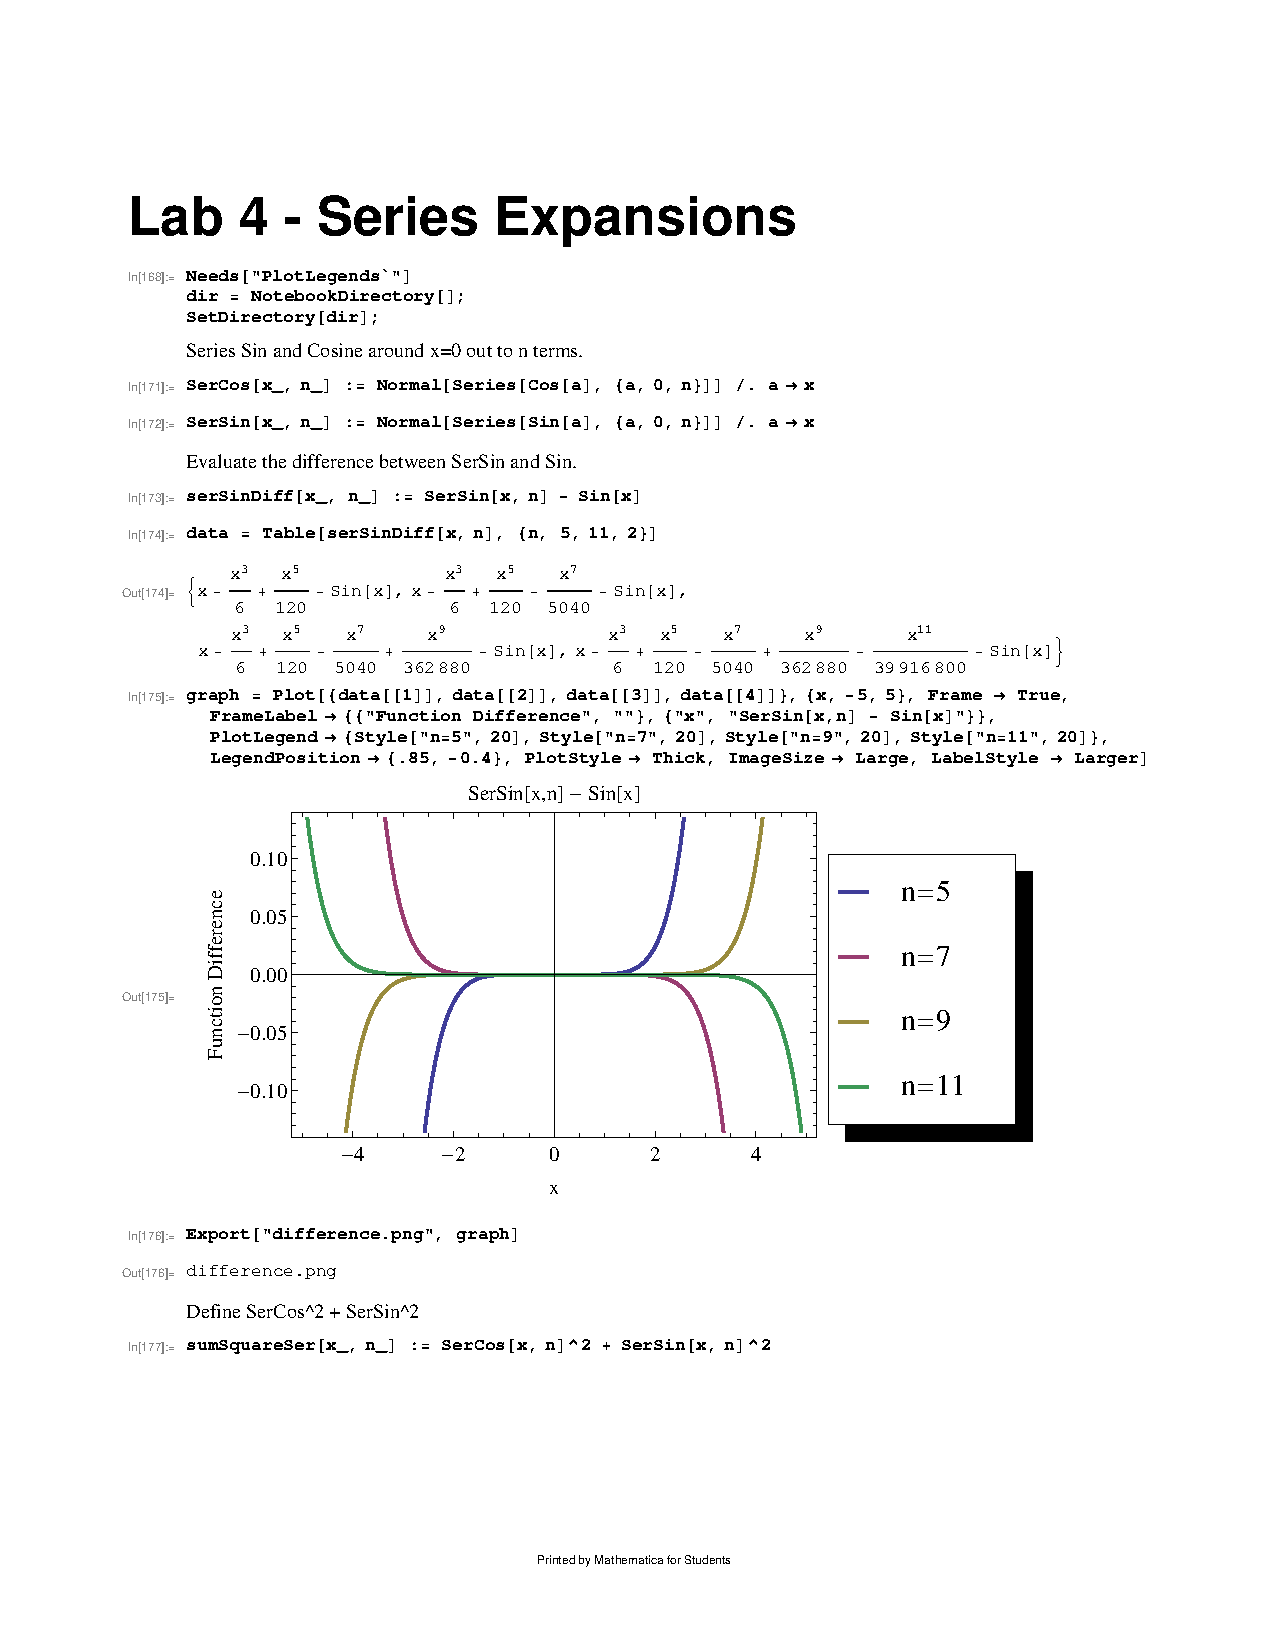
\includepdf[pages={1-4}]{series.pdf}
\end{document}
